\documentclass[10pt,a4paper,oneside]{article}

\usepackage{amsmath, amsthm, amssymb}
\usepackage{graphicx}
\usepackage{caption}
\usepackage{subcaption}
\usepackage{hyperref}
\usepackage{float}

\floatstyle{ruled}
\newfloat{pseudo}{h}{lop}
\floatname{pseudo}{Algorithm}

\usepackage{eulervm}
\usepackage{charter}

\theoremstyle{definition}
\newtheorem*{thm}{Theorem}
\newtheorem{lma}{Lemma}
\newtheorem*{dfn}{Definition}
\newtheorem*{exm}{Example}

\usepackage{color}
\usepackage[usenames,dvipsnames,svgnames,table]{xcolor}

\DeclareMathOperator*{\argmin}{arg\,min}
\DeclareMathOperator*{\argmax}{argmax}

\newcommand{\p}{\mbox{\,.}}
\newcommand{\bD}{\boldsymbol\Lambda}
\newcommand{\R}{\mathbb{R}}
\newcommand{\bm}{\boldsymbol\mu}
\newcommand{\cN}{{\cal N}}
\newcommand{\bs}[1]{{\boldsymbol {#1} }}
\newcommand{\vc}{\textnormal{vec}}
\newcommand{\tab}{\hspace*{5mm}}
\newcommand{\ol}[1]{\overline{#1}}

\theoremstyle{definition}
\newtheorem{theorem}{Theorem}
\newtheorem{definition}{Definition}
\newtheorem{corollary}{Corollary}
\newtheorem{lemma}{Lemma}
\newtheorem{example}{Example}

\title{An Expectation-Maximization Algorithm for the Fractal Inverse Problem}
\date{\today}

% non-indented, spaced paragraphs
\setlength{\parindent}{0.0in}
\setlength{\parskip}{0.1in}

\newcommand{\pb}[1]{\textcolor{OliveGreen}{\small #1 \textsuperscript{[pb]} }}

\begin{document}

\maketitle

\begin{abstract}
\noindent We present a expectation-maximization algorithm to solve the \emph{inverse problem} for iterated function systems (IFS): the task of fitting a fractal model to a given dataset. An IFS is defined by a small number of maps on $\mathbb{R}^H$, the IFS's \emph{components}. A point is sampled from the IFS by starting with some initial point and applying a sequence of randomly chosen components. The central idea of our algorithm is to treat this sequence as a latent variable. If we are given such a \emph{code} for each point in the data, we know which points should map to one another under each transformation of the IFS, allowing us to reconstruct the components. Given the components, we can easily assign codes each point. Iterating these two steps provides us with a basic algorithm to fit an IFS model to data. This idea can be cast as an instance of the Expectation-Maximization (EM) algorithm. Our algorithm  quickly and accurately determines the IFS behind a given dataset. The model reduces to a simple mixture of Gaussians when the data contains no self-similarity. In this treatment, all components are similitudes, but extensions to more general families are simple. 
\end{abstract}

\section{Introduction}
What constitutes a fractal is not precisely defined\footnotemark. The following properties, however, are common to all examples.

First, there is \textbf{self similarity}: a part is a scaled down copy of the whole. See for instance the Sierpinski triangle (fig. \ref{figure:codes}). It consists of three triangular shapes which are scaled down copies of itself. Second, fractals tend to posess \textbf{infinitely fine structure}. 'Zooming in' reveals ever finer detail. In the case of the Sierpinski triangle, we will see the same shape recurring again and again, but other fractals like the Mandelbrot set reveal a great variety of shapes.
Finally, fractals tend to have \textbf{non-integer dimension}. The Sierpinski triangle, for example, has a dimension of $1.58$. 

\begin{figure}[b!]
  \centering
  \begin{subfigure}[b]{0.48\textwidth}
    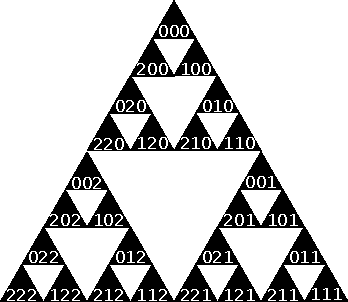
\includegraphics[width=\textwidth]{../img/sierpinski-codes.pdf}
    \caption{}
    \label{fig:sierpinski-codes}
  \end{subfigure}  
  \hspace{0.015\textwidth}
  \begin{subfigure}[b]{0.48\textwidth}
    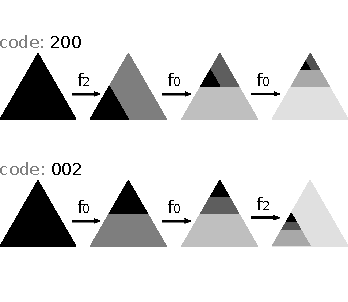
\includegraphics[width=\textwidth]{../img/code-construction.pdf}
    \caption{}
    \label{fig:code-construction}
  \end{subfigure}

  \caption{\small (a) Codes of length three on the Sierpinski triangle and the subsets they code for. (b) The construction of a subset from its code.}
  \label{figure:codes}
\end{figure}

Since the name fractal was coined in the 1970s, fractals have been seen as a potential model for many natural phenomena. Mandelbrot put it as follows in the \emph{The Fractal Geometry of Nature} \cite{mandelbrot1982fractal}:

\begin{quotation}
\small
\noindent Clouds are not spheres, mountains are not cones, coastlines are not circles, and bark is not smooth, nor does lightning travel in a straight line.
\end{quotation}

Fractal geometry has been used in many fields, including physics \cite{mandelbrot1984fractals}, geology \cite{cheng1997multifractal}, biology \cite{goldberger1992fractal} and economics \cite{turiel2003multifractal}.

The greatest problem with fractal analysis has always been the difficulty of finding a fractal model for a given set of data. It may be visually clear that a cloud or a coastline `looks' fractal, and we may be able to determine that it has a non-integer dimension, but how do we get from a dataset to a model? How do we determine the parameters of a fractal-generating model that lead to this particular dataset? Current approaches tend to rely on evolutionary algorithms \cite{deliu1991genetic}. Such techniques take a long time, and it can be difficult to get it to converge to precise parameter values, even if the dataset itself is sampled from a fractal model.
Other approaches are highly domain-specific approaches such as the fractal image compression \cite{hart1996fractal}. Some interesting results have been derived from the method of moments \cite{rinaldo1994inverse} and sampling random transformations from the data \cite{hart1997similarity}, but so far these have not led to a practical algorithm. 

\footnotetext{Mandelbrot originally defined it as a set whose topological dimension differs from its Hausdorff dimension, but retracted this definition, stating that he preferred the word to be not precisely defined.}

A very popular fractal model is the iterated function system (IFS). Many fractals, like the Sierpinski gasket, the Koch curve and the Menger sponge can be seen as IFSs. We will use the following definition:
\begin{definition}
An \emph{Iterated Function System} of order $K$ and dimension $H$ is a pair $(\{f_k\}, \{w_k\})$ of $K$ \emph{components} $f_k$ with $K$ associated\emph{weights} $w_k$. Each component is is a function $f_k: \R^H \to \R^H$, and each weight is a nonnegative scalar, with $\sum_i w_i = 1$. 
\end{definition}
In this paper, all components are similitudes, ie. $f_k$ is defined by a scalar $s_k$, a rotation matrix $R_k$ and a translation vector $t_k$:
\[
f_k(x) = s_kR_k x + t_k \p
\]
The definition can be extended to generic functions and generic metric spaces \cite{hutchinson2000deterministic}, but this formulation is sufficient for our purposes. 

The IFS determines a probability distribution on $\R_H$ in the following way. Let $p_0$ be some initial distribution on $\R^H$ and let $D$ be some nonnegative integer. Sample a point $x_0$ from $p_0$ and pick a random component $f_k$ (according to probability $p(f_k) = w_k$). Let $x_1 = f_k(x_0)$. Sample another random $f_k$ and let $x_2 = f_k(x_1)$, and so on until $x_D$.

There are two basic properties to of IFSs. First, as $D$ grows, the distribution on $x_D$ converges. We call the distribution it converges to the \emph{limit distribution}. Second, the limit distribution is independent of the choice of $p_0$. For formal statements of these properties and their proofs we refer the reader to \cite{hutchinson2000deterministic}.

We can now frame the fractal inverse problem as a problem of statistical parameter estimation: we would like to find the IFS for which the probability of of the data under its limit distribution is maximal. The algorithm we describe is based on the following ideas:
\begin{itemize}
  \item Since the initial distribution doesn't matter, we can choose what we like. We choose the standard multivariate Normal (MVN) distribution $\cN_0$. The benefit of this choice is that every affine transformation of an MVN is itself an MVN. Thus, no matter how high we set $D$, the resulting distribution will always be a mixture of MVNs. 
  \item We assume that each point in the dataset was the result of a length $D$ sequence of applications of the components of the model. We cast this sequence---called a \emph{code} hereafter---as a latent variable in our model. Each code $c$determines an \emph{endpoint distribution}, and each endpoint distribution is an MVN $\cN_c$.
  \item  Given the IFS that generated our data, it is a simple matter to find the most likely code for each point $x$. Conversely, if we know the most likely code for each point, we can determine which points in the dataset should map to one another, under a particular component $f_k$. This correspondence allows us to reconstruct $f_k$.    
\end{itemize}

We make the correspondences in the last point probabilistic: instead of assigning each point its most likely code, we compute a \emph{responsibility} that each possible component takes for the point. This is the posterior probability of the component given the point: $p(c \mid x) \propto p(x \mid c) p(c)$, where $p(x\mid c) = N_c(x)$ and $p(x) = \prod_{s \in c} w_s$. This is the \emph{expectation} step of the algorithm. The \emph{maximization} step, optimizing the IFS model given these probabilities is detailed in the body of the paper. 

Note that finding a code corresponding to a particular endpoint can be counter-intuitive, as the first component applied determines the location at the smallest scale, and the last component applied determines the location at the largest scale. Figure~\ref{figure:codes} provides an illustration.

We show in Section~\ref{section:experiments} that our algorithm quickly reconstructs many known fractals, such as the Sierpinski gasket and the Koch curve. We also apply the algorithm to some datasets sampled from images, showing that, in principle, it can find approximations of naturally occurring fractals, that are not specifically IFSs.   

\subsection{Preliminaries}
\paragraph{Measures and transformations} Let $\{x_i\}_{i\in[1,N]}$, $x_i\in\R^H$ be our dataset. Let $X$ be the $N\times H$ matrix with $x_i$ as its columns. All vectors are column vectors.  

Let $1_L$ be the length-$L$ vector with $1$ at all indices. Such vectors are useful tools in dealing with matrices, for instance, the sum of the elements of the $K \times L$ matrix $M$ can be expressed as ${1_K}^T M 1_L$, while its marginal vectors are $({1_K}^T M)^T$ and $M 1_L$. Let $0_L^j$ be the length-$M$ vector with element $j$ $1$ and all others $1$. This vector functions as a row- or column-selector, eg. $X 0^j_N = x_i$.

Let $v(X)$ be a probability distribution with $X \subseteq \R^H$. Let $f_{t, A}(x) = Ax + t$ be an invertible affine transformation represented by a vector $t$ and a matrix $A$. Then the transformation of $v$ by $f_{t, A}$ is defined by the relation $f_{t, A}(v)(X) = v({f_{t, A}}^{-1}(X))$. Let $v(x)$ be the density function of  the measure $v$ (with respect to the Lebesgue measure). Then the density function of the measure $f_{t, A}(v)$ is $f_{t, A}(v)(x) = |A^{-1}| v({f_{t, A}}^{-1}(x))$.

A multivariate normal distribution (MVN) on $\R^H$ is determined by a mean $\mu \in \R_H$ and a covariance matrix $\Sigma \in \R^{H\times H}$. Its probability density function is:
\[
\cN(x \mid \mu, \Sigma) = (2\pi)^{-\frac{H}{2}}|\Sigma|^{-\frac{1}{2}} \exp \left [-\frac{1}{2} \left \| (x-\mu)^T\Sigma^{-1}(x-\mu) \right\|^2\right] 
\]
We will call the MVN with $\mu = 0$, $\Sigma = I_H$ the standard multivariate normal distribution, or $\cN_0$. A \emph{spherical MVN} has $\Sigma = sI$ for some scalar $s$. Let $x$ be random variable with $x \sim \cN(\mu, \Sigma)$, then $f_{t, A}(x) \sim \cN(t + A\mu, A\Sigma A^T)$. 

A \emph{rotation matrix} $R$ is a matrix with $R_R = I$ and $|R| = 1$. A \emph{similitude} (or rigid transformation) on $\R^H$ is a transformation defined by a rotation matrix $R \in \R^{H\times H}$, a translation vector $t \in \R^H$ and uniform scaling $s \in R$: $f_{t, R, s}(x) = sRx + t$. 
The inverse of a similitude is also a similitude: ${f_{s, R, t}}^{-1}(x) = f_{\frac{1}{s}, R^T, -\frac{1}{s}R^Tt}(x)$.

$f_{s, R, t}(\cN_0)$ is a spherical MVN with mean $t$ and covariance $s^2I$. Transforming a generic spherical MVN by a similitude can be cast as the transformation of $\cN_0$ by two similitudes:
\begin{align}
f_{t, R, s}(\cN_{t_0, {s_0}^2 I})(x) &= f_{t, R, s}(f_{t_0, R_0, s_0}(\cN_0))(x) \notag \\
&=  (2\pi)^{-\frac{H}{2}} \frac{1}{ss_0} \exp \left[- \frac{1}{2{s_0}^2s^2}\left\| x - (s R t_0 + t)\right \|^2\right] \label{line:inverse}
\end{align}
\paragraph{The EM Algorithm} \cite{dempster1977maximum}
Let $p(X\mid Z, \theta)$ be probability distribution with parameters $\theta$ and latent variables $z$. The most common example is a mixture of MVNs: in this case $\theta$ contains the parameters of $K$ MVNs together with a weight $w_k$ for each, and $Z$ is a matrix whole columns $z_i$ determine which component is responsible for $x_i$: ie. if component $k$ is responsible, then $z_ki$ is 1 and all other $z_ki$ are 0.

The maximum likelihood parameters for a dataset $X$ are determined by 
\[
\argmax_{\theta} \ln p(X|\theta) = \argmax_{\theta} \ln \sum_Z p(X|Z, \theta)p(Z) 
\]
where the sum is over all possible values of $Z$. The value in side the sum is the \emph{complete-data likelihood} $p(X, Z\mid \theta)$. In the mixture-of-MVNs example, there are $K^N$ possibilities for $Z$, making this sum intractable for practical data. 
 
The intuition behind EM is to maximize $\theta$ with respect to our best guess for $Z$ and vice versa. Let $\theta^\text{old}$ be our current best guess for the parameters. We first optimize $p(Z\mid X, \theta^\text{old})$, the posterior on the latent variables. Note that, in the MVN example, we can represent this as an $N\times K$ matrix $Z$ with $Z_{ij} = p(j\mid x,\theta) = N^\text{old}_j(x) w_j$. This is known as the \emph{expectation} step.

We then determine the expectation of the logarithmic complete-data likelihood under  our posterior $p(Z|X, \theta^\text{old})$ as a function of $\theta$.
\[
Q(\theta) = \sum_Z p(X|Z, \theta)p(Z) \ln p(X, Z \mid \theta)
\]  
Note that the complete-data likelihood is now inside the logarithm. We optimize this $Q$-function, with respect to $\theta$ to get $\theta^\text{new}$, our new best guess for the parameters. This is known as the \emph{maximization} step. The EM algorithm iterates the two steps until the algorithm converges.

\section{The IFS model}

\begin{figure*}[t]
  \center
  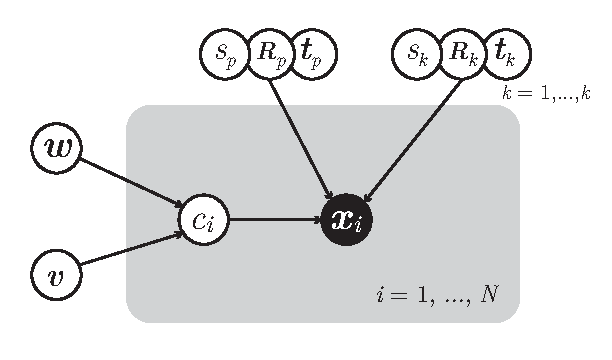
\includegraphics[width=0.7\textwidth]{../img/factor-graph.pdf}
  \caption{A graphical model, illustrating the components of the IFS model. The gray box is a plate, representing a repetition of the nodes inside the box for each datapoint. The black node represents the observed data.}
  \label{figure:ifs-diagram}
\end{figure*}

The complete IFS model is illustrated in Figure~\ref{figure:ifs-diagram}. It consists of:
\begin{description}
\item[the component weights $w$] This is a vector of $K$ non-negative real values, with $\sum_k w_k = 1$. Each weight determines the probability of its associated component being chosen at each iteration of the IFS.
\item[the depth  priors $v$] The number of times the IFS is iterated for each point. $v$ is a vector representing a categorical distribution on $[0,D]$, from which the length of the code $c$ is sampled. 
\item[the components $f_k = \{s_k, R_k, t_k\}$] $K$ similitudes. 
\item[The post-transformation $s_p, R_p, t_p$] The parameters a single \emph{post-transformation}. This transformation is applied once to all sampled points.
\item[The code $c_i$] An ordered sequence $c_i = \langle c_{i1}, \ldots, c_{id} \rangle$. Each element of the code is an integer in $[1,K]$ representing a component. 
\item[The data $x_i$] This is the point after the post-transformation is applied: ie. the observed data.
\end{description}

To sample a point $x_i$ from this model we first sample a depth $d$ with $p(d=a) = v_a$. We then sample a sequence $c_i$ of $d$ components $c_{i1}, \ldots, c_{dj}$ with each $c_ij \in [1,K]$ chosen independently with $p(c_ij = a) = w_a$. We then create the composite function $f = f_p \circ f_{c_{i1}} \circ \ldots \circ f_{c_{id}}$ and sample $x$ from $f_(N_0)$.

Giving the model a variable depth has several advantages. First, it makes the model a generalization of good fall-back models. with $v_0 = 1$, the model becomes a spherical multivariate Gaussian. With $v_1 = 1$, the model becomes a mixture of spherical Gaussians.\footnotemark Since each point has its own depth, the full model is a mixture over all these models, and the deeper IFS models. If the data is not self similar, or only partially self similar (like an IFS model with ourliers), the lower depth parts of the mixture can capture this.

This also allows the EM search a `gentle start'. In the limit, most IFSs have a support with lower dimension than the embedding dimension of the data: ie. almost all of $\R^H$ has probability zero. This means that even if the model fits the source of the data perfectly, the slightest addition of noise will make the entire likelihood zero. It also means that a minute change in parameters can mean the difference between the maximum likelihood, and likelihood zero. In effect, for high values of $d$, the fitness landscape becomes very jagged. 

The variable depth provides an automatic defense: if such a drop occurs, the lower models, whose fitness landscape is smoother, automatically get a higher posterior, smoothing out the fitness landscape for the complete mixture. As the search converges to the correct model, the depth prior becomes more weighted towards the higher depths.

However, the variable depth also creates a problem: while any transformation of an IFS by a similitude is also an IFS, how the components of the original IFS are transformed depends on the parameter $D$. Imagine a dataset sampled from a Sierpinski gasket translated away form the origin. We have good models at every depth for this data, but their components are different. Only if the data is centered do the components coincide for all depths, but how the data should be centered depends on the parameters of the IFS. For this reason, we introduce the\emph{post-transform}:we learn a centered IFS, and transform the full limit distribution to fit the data.   

\footnotetext{To generalize to non-spherical MVNs and mixtures over non-spherical MVNs, the component family should be extended to positive definite affine functions. This extension is discussed in the conclusion.}

\section{The EM algorithm for IFS models}

We will use the notation $[1,K]^d$ to refer to the set of all length-$d$ codes. Let $[1,K]^{[a,b]} = \bigcup_{d \in [a,b]} [1,K]^d$. Thus, the set of all codes, including the empty code, is $[1, K]^{[0, D]}$. For every code $c_j$ in this set, we have 
\begin{align*} 
p(x \mid c_j) &= \cN(x \mid \mu_j, \Sigma_j) \\
p(c_j) &= p(d) \prod_i p(c_j) = v_{|c_j|}\prod_{i \in c_j} w_{i}
\end{align*}

Where $\mu_j$ is the mean corresponding to $f_j(\cN_0)$ with $f_j = f_p \circ f_{c_{j1}} \circ f_{c_{j2}} \circ \ldots \circ f_{c_{jd}}$, and $\Sigma_j$ is the covariance matrix $f_j(\cN_0)$.

\subsection{The latent variables}

The responsibilities for an MVN mixture model are well-known. Let $M = |[1, K]^{[0, D]}|$ and let $P$ be an $N\times M$ matrix with: 
\[
P_{ij} = p(c_j \mid x_i) = \frac{p(x_i\mid c_j) p(c_j) }{\sum_{a \in [1,K]^{[0, D]}} p(x_i\mid c_a) p(c_a)} \p 
\]
We also create a specific matrix for each $f_k$ for purposes that will become clear in the next section. Let $M = |[1, K]^{[0, D-1}]|$, and let $P^k$ be an $N \times M$ matrix with: 
\[
P_{ij}^k = p(k.c_j \mid x_i) = \frac{p(x_i\mid k.c_j) p(k.c_j) }{\sum_{a \in [1,K]^{[0, D]}} p(x_i\mid c_a) p(c_a)} 
\]
where $k.c_j$ is the code $\langle k, c_{j1}, \ldots, c_{j|c|}\rangle$. Note that this is a sub-matrix of $P$.

Note that the size of these matrices will grow very fast with $D$, and most of its values will be practically indistinguishable from $0$ when normalized. For this reason, it may be advisable to set all but the largest values to $0$, and store the matrix in a sparse datastructure. For our experiments, such optimizations were not necessary.

\subsection{The parameters}

Let $F^\text{old}$ be the model we used to compute the responsibilities. Our $Q$-function is:
\begin{align*}
Q(F) &= \sum_{i} p(z_i \mid x_i, F^\text{old}) \ln p(x_i \mid z_i, F) p (z_i \mid F) \\
     &= \sum_{i=1,j=1}^{N, M} P_{ij} \ln \cN_j(x) \;v_{|c_j|}\; \prod_{a\in c_j}w_a \,\,\, \text{with } M = |[1,K]^{[0,D]}|
\end{align*}

For clarity of notation, when optimizing for a certain subset of the parameters $q$ (such as the depths, weights or parts of the components) we will write $Q(q)$, and omit any terms that are constant with respect to $q$. We may also omit any constant multiplier of the whole function.

To find the optimal depth we solve $\partial Q(v)/\partial v$, using a Lagrange multiplier to enforce that $v$ sums to one, which gives us:
\[
\hat v_d = \frac{p_d}{\sum_i p_i} \,\,\text{with } p_d = \sum_{j: |c_j| = d} P_{ij}
\]

\paragraph{The components $f_k$ and weights $w_k$}

Even with the simplifications of the EM algorithm $Q$ is very difficult to optimize for $f_k$ and $f_p$. We must find $K$ maps and weights, and a post-transformation $f_p$, such that all the $M$ endpoint distributions, provide maximal likelihood to their assigned points. The problem is that each term in $Q$ is a complicated mix of multiple components.

To make the optimization of $Q$ practical, we simplify the task in two ways. First, we optimize $f_p$ and $(\{f_k\}, \{w_k\})$ separately, taking the parameters not being optimized from $F^\text{old}$. Let $Y = {f_p^\text{old}}^{-1}(X)$. Second, we simplify the $Q$ function as follows: 

\begin{align*}
Q(\{f_k\}, \{w_k\}) = \sum_k \sum_{i=1,j=1}^{N, M} & p(k.c_j \mid x, F^\text{old}) \ln f_p f_k(\cN_{j})(x_i) p^{\text{old}}(c_j) p(k)\\ & \hfill \text{with } M = |[1,K]^{[0, D-1]}|  \\
= \frac{1}{s^\text{old}_p}\sum_k \sum_{i, j} &P^k_{ij} \ln \left[ f_k(\cN_{j})(y_i) \; v_{|c_j|+1} p(c_j) \; w_k \right]\p
\end{align*}
We then \emph{approximate} all elements indexed by $j$, so that of all the transformations in each code, only the last one functions as an argument of $Q$. We approximate $\cN_j$ by fitting a maximum likelihood spherical MVN to the data weighted by $P^k1_M$: that is, the part of the dataset that $\cN_j$ was responsible for under the old model. This gives us $\cN_j = f_{s_j, I, t_j}(\cN_0)$ with
\[
t_j = \frac{YP^k0_M^j}{P^k0_M^j 1_M} \;\;\;\;\; s_j = \sqrt{\frac{\sum_i \|P^k0_M^j - t_j\|^2 }{({1_M}^TP^k)_j}} \p
\]
That is, $t_j$ and $s_j$ are the weighted mean and weighted standard deviation respectively. Arranging the different $t_j$ as the columns of a matrix $T^k$, we get 
\begin{align}
T^k = Y(P^k / (1_N{1_M}^TP^k)) \label{line:tk}
\end{align}
where the division is element-wise. $p(c_j)$ becomes a term independent of any parameters, so we need not approximate it. This gives us:
\begin{align*}
Q(f_k, w_k) &= \sum_{i, j} P^k_{ij} \ln f_k(\cN_j)(y_i) + \sum_{i, j} P^k_{ij} \ln w_k  
\end{align*}
Finding $w_k$ follows the same principle as the depths. We find:
\[
\hat w_k = p^k / \sum_{i} p^i \p
\]
with $p^k = {1_N}^TP^k1_M$, the sum of the elements of $P^k$.

If we isolate $f_k$, the problem is very similar to the one solved to construct the Coherent Point Drift (CPD) algorithm \cite{myronenko2010point}: transform a set of MVNs to maximize the likelihood of a dataset, with responsibilities of components for datapoints given. The main difference is that in our situation each component $N_j$ has its own variance. We follow the same approach, and as we shall see, the solutions for our problem are very similar to those of the CPD algorithm.

Using Equation~\ref{line:inverse} from the preliminaries, we can rewrite $Q(f_k)$ as a mixture of transformations of $\cN_0$:
\begin{align*} 
Q(s_k, R_k, t_k) &= - p^k\ln s_k - \sum_{i, j} P^k_{ij} \frac{1}{2{s_j}^2{s_k}^2} \left\|y_i-t_k - s_k R_k t_j \right\|^2 
\end{align*}
where $s_j$, $R_j$ and $t_j$ are the parameters of the similitude $f_p \circ c_{j1} \circ \ldots \circ c_{jd}$. 

To find the optimal translation $t_k$, we solve $\partial Q(t_k)/\partial t_k = 0$, which yields, in matrix notation:
\begin{align*}
\hat t_k &= \frac{1}{p^k_z}YP^kZ1_M - \frac{1}{p^k_z}s_kR_kT^kZ{P^k}^T1_N = y^k - s_kR_k t^k
\end{align*} 
where $T^k$ is the matrix with $t_j$ as its columns, $Z = \text{diag}({s_1}^{-2}, \ldots, {s_M}^{-2})$ and ${p^k_z} = {1_N}^TP^kZ1_M$, the sum of the elements of the matrix $P^kZ$. Thus $\hat t_k$ is the difference between a weighted mean of the data $y^k$ and a weighted mean of the endpoint means $t_j$, scaled and rotated, where in both cases, the matrix  $P^kZ$, normalized to sum to one, determines the weights. Note that this is not a complete solution, since it still depends on $s_k$ and $R_k$. We can, however, plug $\hat t_k$ back into the $Q$-function to optimize for $R_k$.

Finding the optimal rotation matrix $R_k$ is more complex than simply finding the derivative and setting it equal to zero, since we have the constraint that $R_k$ is orthogonal and has determinant $1$. Luckily, a similar problem was solved in \cite{umeyama1991least} and \cite{myronenko2010point}. To use this solution, the objective function must be rewritten to the form $\text{tr}(A^TR_k)$ for some $A$. We fill in $\hat t_k$, and reduce to
\[ 
Q(R_k) = \text{tr}\left(\left[\ol{Y}^kP^kZ{\ol{T}^k}^T\right]^TR_k\right) 
\]
with 
\begin{align*}
\ol{Y}^k &= Y - y^k {1_N}^T\\
\ol{T}^k &= T^k - t^k {1_M}^T\\
\end{align*}
By \cite[Lemma~1]{myronenko2010point}, the optimal $R_k$ can be derived from the singular value decomposition (SVD) of $A=Y^kP^kZ{T^k}^T$. If $A = USV^T$, with $U$, $S$ and $V$ defined as normal for the SVD then we have $\hat R_k = U \;\text{diag} (1, \ldots, 1, |UV^T|)\; V^T$.

Finally, we derive the scaling parameter $s_k$ by filling in $\hat t_k$ and solving $\partial Q(S_k)/\partial s_k$. We get:

\begin{align*}
0 &= {s_k}^{-2}\;\text{tr}({\ol{Y}^k}^T\text{diag}(P^kZ1_M)\ol{Y}^k) + {s_k}^{-1}\;\text{tr}(\ol{T}^kZ{P^k}^T{\ol{Y}^k}^TR_k) -p^k \p
\end{align*}
This is a quadratic polynomial in ${s_k}^{-1}$, which we can solve and invert to find $\hat s_k$.

\subsection{The post transform: $s_p$, $R_p$, $t_p$} Let $M = \left |[1,K]^{[0,D]}\right|$ The $Q$-function becomes:
\begin{align*}
Q(s_p, R_p, t_p) &= \sum_{i=1,j=1}^{N,M} p(c_j\mid x_i) \ln f_p(N_j)(x_i) p(c_j) \\
&= - p\ln s_p  - \frac{1}{2 {s_p}^2} \sum_{i, j} {s_j}^{-2} P_{ij} \| x - t_p -s_pR_pt_j \|^2 \\
\end{align*}
where $p = {1_N}^T P 1^M$ and $s_j$ and $t_j$ can be derived from the optimal components, as determined above. Note that $j$ now iterates over a larger set of codes.

The form of the $Q$ function is the same as the ones we used to derive the optimal components $s_k, R_k, t_k$. We follow the same derivations and get: 

\begin{align*}
\hat t_p &= \overline{x} - s_pR_p\overline{t}\\
\hat R_p &= U\;\text{diag}(1, \ldots, 1, |UV^T|)\;V^T & \text{with } USV = \text{svd}(A), A = \ol{X} P Z {\ol{T}}^T \\
\end{align*}
with 
\begin{align*}
\ol{x} &= ({1_N}^TPZ1_M)^{-1} XPZ1_M & & \ol{t} = ({1_N}^TPZ1_M)^{-1}TZP^T1_M\\
\ol{X} &= X - \overline{x}{1_N}^T & &\ol{T} = T - \overline{t} {1_M}^T\\
Z &= \text{diag}({s_1}^{-2}, \ldots, {s_M}^{-2})\\
\end{align*}

Finally, for $s_p$, we solve
\[
0 = {s_p}^{-2}\text{tr}(\ol{X}^T\text{d}(PZ1_M)\ol{X}) + {s_p}^{-1} \text{tr}(\ol{T}ZP^T\ol{X}^TR_p) - p
\]

\begin{pseudo}[th]
\caption{One iteration of the EM algorithm for fitting a fractal model.}
{
Given: a dataset $X$, a number of components $K$, a maximum depth $D$. \\

$C \leftarrow [0,K]^{[0, D-1]}$, $M \leftarrow |C|$ \emph{\# the set of all codes of length up to $D$} \\
\emph{\# Expectation step}\\
$P_{ij} \leftarrow N_j(x_i) p(d) \prod_{c \in [1,K]^d} w_c$  \\ 
Normalize $P$ so that $P1_M = 1_N$ \\
\textbf{for each} $k \in [1,K]$: \\
\tab Let $P^k$ be the submatrix of $P$'s columns $j$ such that $c_{j1} = k$\\
\\
\emph{\# Maximization step} \\
$Y \leftarrow {f^\text{old}_p}^{-1}(X)$\\
for all $d$, $v_d \propto \sum_{j : |c_j| = d} P_{ij} $\\
\textbf{for each} $k \in [1,K]$: \\
\tab $w_k \leftarrow {1_N}^T P^k 1_M / \sum_i {{1_N}^T P^i 1_M}$\\
\tab $y^k \leftarrow {p^k}^{-1}YP^kZ1_M, \,\,\, t^k \leftarrow {p^k}^{-1} T^kZ{P^k}^T 1_N$\\
\tab $\ol{Y}^k \leftarrow Y + y^k{1_N}^T$, \,\,\, $\ol{T}^k \leftarrow T^k + t^k{1_M}^T$\\
\tab $Z \leftarrow \text{diag}({s_1}^{-2}, \ldots, {s_M}^{-2})$\\
\tab $U,S,V^T \leftarrow \text{svd}(\ol{Y}^kP^kZ{\ol{T}^k}^T)$\\ 
\tab $R_k \leftarrow U\;\text{diag}(1,\ldots,1,|UV^T|) V^T$ \\
\tab $s_k$: solve ${s_k}^{-2}\; \text{tr}({\ol{Y}^k}^T\text{d}(P^kZ1_M)\ol{Y}^k) + {s_k}^{-1}\;\text{tr}(\ol{T}^kZ{P^k}^T{\ol{Y}^k}^TR_k) = 0$ \\
\tab $t_k \leftarrow y^k - s_k R_k t^k$ \\

$C \leftarrow [0,K]^{[0, D]}$, $M \leftarrow |C|$\\
$X' \leftarrow X - \overline{x}{1_N}^T$, $T' \leftarrow T + \overline{t}{1_M}^T$\\
\tab $Z \leftarrow \text{diag}({s_1}^{-2}, \ldots, {s_M}^{-2})$\\
$U,S,V^T \leftarrow \text{svd}(X'PZ{T'}^T)$\\ 
$R_p \leftarrow U\;\text{diag}(1,\ldots,1,|UV^T|) V^T$ \\
$s_p$: solve ${s_p}^{-2}\text{tr}(X'PZ1_NX'+ T'Z{P}^T1_MT') - s_p^{-1} \text{tr}(ZP^T{x'}^TT') -2p = 0$ \\
$t_p \leftarrow \overline{x} - s_pR_p\overline{t}$ \\
}
\end{pseudo}

\subsection{Dealing with singularities}

In the EM algorithm for MVN mixtures, there is a danger that the algorithm becomes stuck in a situation where one or more of the components do not have responsibility for any part of the data, or for only a single point. In this case, the covariance matrix for such components cannot be computed, and the algorithm must be reset in some way.

In the IFS algorithm a similar thing can happen, causing one or more of the mtrices $P^k$ to become low-rank. In this case, the SVD decomposition required to find $R_k$ cannot be computed. When this happens, we use the following strategy: we remove the undetermined component, and for each one we \emph{split} one of the well-determined components. Let $f_a = (s_a, R_a, t_a)$ with weight be the well-determined component and $f_b$ be the singleton component. We resolve the situation by setting:
\begin{align*}
f_a \leftarrow (s_a, R_a, t_a + \epsilon_a)\\
f_b \leftarrow (s_a, R_a, t_a + \epsilon_b) 
\end{align*}
where $\epsilon_a, \epsilon_b$ are vectors with elements randomly drawn from $\cN(0, \sigma)$, where we use $\sigma = 0.001$ in all experiments. The weight $w_a$ is distributed equally over the components $f_a$ and $f_b$ and the weight vector is re-normalized.
 
The rationale is easiest to understand if we take $v_1=1$ and view the model as a mixture of Guassians. In that case, the well-determined components cover all the data. By splitting $f_a$, and adding some small noise, the points formerly `claimed' by $f_a$ will now be distributed approximately evenly between $f_a$ and $f_b$. 

\section{Results}
\pb{subsampling}
\pb{initial models}

\label{section:experiments}

\subsection{Synthetic distributions}

\pb{sierpinski, koch-2, ball}

\subsection{Images}

\pb{Sunflower}

\subsection{Higher-dimensional data}

\pb{spherical-MOG, full MOG, IFS, three datasets}

\section{Discussion}

We have introduced a new algorithm for the induction of fractal models. To our knowledge this is the first such algorithm that does not use a general-purpose optimization technique like genetic algorithms. 

In the introduction we mentioned the intuitive motivation for the algorithm that given the codes for each point, we can consbtruct paired lists of points for each component such that the first list should map onto the second, reducing the inverse problem to the absolute orientation problem, as solved in \cite{umeyama1991least}. The reader may wonder if we have strayed from this original idea in our EM treatment, since our $Q$-function do not seem to map points onto one, but rather endpoint distributions onto points. However, since our simplification of the $Q$-function in Equation~\ref{} estimates these endpoint distributions from a re-weighted dataset, we can substitue these, and show that there we are in effect building an $N \times N$ matrix ${\cal P}^k$ and solving a weighted version of the absolute orientation problem, mapping every point $x_i$ in the data onto every other point $x_j$ with weight ${\cal P}^k_{ij}$. This is proved in the appendix. 

Similitudes were chosen as a nice balance between expressiveness and parameter complexity. More general function classes are certainly possible, although deriving the maximization step analytically may not be possible for these. For instance, if we allow generic, affine  functions, defined by a translation $t$ and a matrix $A$, we find a derivative of the form $\frac{\partial Q}{\partial A} |A^{-1}| + cA$. This is difficult, if not impossible to solve analytically, although if we restrict $A$ to be positive definite, we can see that the problem is convex, so that we can easily solve it numerically.

An alternative approach would be to use a variational Bayesian algorithm instead of an EM algorithm. If a variational algorithm exists for the desired function class, it should be straightforward to plug these into a general variational algorithm for iterated function systems. Such an approach would also avoid the problem of singularities, and it would allow some tuning of the algorithm through the selection of priors. We consider this a promising direction for future research.

Many natural fractal phenomena are not precisely captured by iterated functions systems. Coastlines trees and clouds are self-similar, but in a much more random manner than IFSs can describe. One solution takes the form of an extension to random iterated function sytems, as described in \cite{hart1996fractal}. Here, at each application the IFS is itself chosen at random from a distribution on IFSs. Another option would be to manually add domain knowledge about the data into the model, for instance specific knowledge about the development of clouds or the growth of trees. In both cases, we believe the EM algorithm provides a basic template for a solution: the main issue is that of finding the specific choices made inside the model to arrive at each point in the dataset. By casting this sequence of choices as a latent variable, and applying Bayes rule (either using EM or a variational approach), we divide and conquer: we cannot solve the problem as a whole, but we can find the latent variables given the parameters, and the parameters given the latent variables.

\bibliographystyle{siam}
\bibliography{fractal}

\appendix

\section{Derivations}

Transforming a generic spherical MVN by a similitude can be cast as the transformation of $\cN_0$ by two similitudes:
\begin{align*}
f_{t, R, s}(\cN_{t_0, {s_0}^2 I})(x) &= f_{t, R, s}(f_{t_0, R_0, s_0}(\cN_0))(x) = f_{ sRt_0+t, RR_0,ss_0}(\cN_0)(x) \\
&= \frac{1}{ss_0} \cN_0\left(\frac{1}{ss_0} {R_0}^T R^T x - \frac{s}{ss_0} {R_0}^Tt_0 - \frac{1}{ss_0} {R_0}^TR^Tt \right) \\
&= \frac{1}{ss_0} \cN_0\left(\frac{1}{ss_0} x - \frac{1}{s_0} {R}t_0 - \frac{1}{ss_0} t \right) \\
&= \frac{1}{ss_0} \cN_0\left(\frac{1}{ss_0} {R_0}^T R^T x - \frac{s}{ss_0} {R_0}^Tt_0 - \frac{1}{ss_0} {R_0}^TR^Tt \right) \\
&=  (2\pi)^{-\frac{H}{2}} \frac{1}{ss_0} \exp \left[- \frac{1}{2{s_0}^2s^2}\left\| x- t - s R t_0 \right \|^2\right]
\end{align*}

\paragraph{The depth $v$ and weights $w$} For the depth priors $v$, the $Q$-function, with constant terms omitted, reduces to:
\begin{align*}
Q(v) &= \sum_{i,j} P_{ij} \ln v_{|c_j|} \\ 
&= \sum_{d \in [0,D]} \sum_{j: |c_j| = d} P_{ij} \ln v_d = \sum_{d \in [0,D]} \left[\sum_{c: |c| = d} P_{x, c}\right] \ln v_d\\
&= \sum_{d \in [0,D]} p_d \ln v_d \;\;\text{with $p_d = \sum_{c: |c| = d} P_{x, c} $}  \\
\end{align*}
For $v$, we have the additional constraint that $\sum_d v_d = 1$, which we can take into consideration with lagrange multipliers, giving us the objective function ${\cal L}(v, \lambda) = p_d/v_d - \lambda\sum_d v_d - \lambda$. We differentiate and set equal to zero, giving us the equations $p_d/v_d - \lambda = 0$ amd $\sum_i v_i -1 =0$. Solving these gives us:
\[
\hat v_d = \frac{p_d}{\sum_i p_i}
\]

Finding $w_k$ follows the same principle as the depths. The $Q$-function reduces to:
\[
Q(w) = \sum_{k} p_k \ln w_k
\]

Using Lagrange multipliers to incorporate the constraint that $\sum_i w_i = 1$, we find
\[
\hat w_k = p^k / \sum_{i} p^i \p
\]

\paragraph{The translations $t_k$} The optimal translation can be found by straightforward differentiation:
\begin{align*}
\frac{\partial Q(t_k)}{\partial t_k} &= 
- \sum_{i,j} P_{ij}^k \frac{1}{{s_j}^2{s_k}^2}\frac{\left \|  y_i - t_k - s_kR_kt_j \right\|^2}{\partial t_k}
\\
&= \sum_{i,j} P_{ij}^k \frac{1}{{s_j}^2{s_k}^2} \left(y_i - t_k - s_kR_kt_j\right)^T \\
\end{align*}

This sum represents a row vector, which we transpose to get a column vector, and set equal to zero to get $\hat t_k$:
\begin{align*}
0 &= \frac{1} {{s_k}^2} \left (\sum_{i,j} P^k_{ij} {s_j}^{-2} y_i  - \sum_{i,j} P^k_{ij} {s_j}^{-2} t_k - s_kR_k \sum_{i,j} P^k_{ij} {s_j}^{-2} t_j\right) \\
\end{align*}

Let $Z = \text{diag}({s_1}^{-2}, \ldots, {s_M}^{-2})$, we can then rewrite to matrix notation:
\begin{align*}
\hat t_k &= \frac{YP^kZ1_M - s_kR_k\;T_j(P^kZ)^T1_N}{{1_N}^TP^kZ1_M} 
\end{align*} 

\paragraph{The rotations $R_k$}
\begin{align*} 
Q(R_k) &= - \frac{1}{2}\sum_{i,j} P^k_{ij} \frac{1}{{s_j}^2{s_k}^2} \left\| y_i - t_k - s_kR_k t_j \right\|^2\\
&= - \frac{1}{2}\sum_{i,j} P^k_{ij} {s_j}^{-2} \left\| \left(y_i - y^k\right) - s_kR_k \left(t_j-t^k\right) \right\|^2 \p 
\end{align*}
Let ${y^k_i} = y_i - y^k$ and ${t^k_j} = t_j - t^k$, ie. mean-centered versions of the data points and the component means. Let $Y^k$ and ${T^k}$ be the corresponding matrices with these vectors as columns. We multiply out the inner product to get
\begin{align*}
Q(R_k) &= - \frac{1}{2}\sum_{i,j} P^k_{ij} {s_j}^{-2} \left[ {y_i^k}^T{y_i^k} - 2 s_k {y_i^k}^TR_k{t_j^k} + {t_j^k}^T{t_j^k} \right] \\
\end{align*}
from which we remove the terms and global factors that are independent of $R_k$:
\begin{align*}
Q(R_k)&= \sum_{i,j} P^k_{ij}\; {s_j}^{-2}\; {y_i^k}^TR_k{t_j^k}
\end{align*}
Which in matrix notation becomes:
\begin{align*} 
Q(R_k) &= \text{tr}((P^k Z)^T {Y^k}^TR_kT^k) = \text{tr}(T^k Z {P^k}^T{Y^k}^TR_k) = \text{tr}([Y^kP^kZ{T^k}^T]^TR_k) \p
\end{align*}
Where we use the fact that $\text{tr}(A^TB) = \sum_{i,j}(A\circ B)_{ij}$ and the fact that the trace is invariant under cyclic permutations.

\paragraph{The scaling $s_k$}
We derive the scaling by filling in $\hat t_k$ and solving for $\partial Q(S_k)/\partial s_k$.
\begin{align*}
\frac{\partial Q(s_k)}{\partial s_k} &=  \frac{- p^k \ln s_k - \sum_{i,j} P^k_{ij} \frac{1}{2{s_j}^2} \left\|y_i - t_k - s_k R_k t_j \right\|^2}{\partial s_k}\\
\frac{\partial Q(s_k)}{\partial s_k} &= - p^k {s_k}^{-1} - \sum_{i,j} P^k_{ij} \frac{1}{2{s_j}^2} \left(-{s_k}^{-3} {y^k_i}^T y^k_i + {s_k^{-2}} {y^k_i}^TR_kt_j^k + {s_k}^{-3}{t_j^k}^T t_j^k\right) \\
&= - p^k {s_k}^{-1} + {s_k}^{-3} \frac{1}{2}\sum_{i,j} P^k_{ij} 2{s_j}^{-2} {y^k_i}^T y^k_i \\ 
& - {s_k}^{-2} \frac{1}{2}\sum_{i,j} P^k_{ij} 2{s_j}^{-2} {y^k_i}^TR_kt_j^k - {s_k}^{-3} \frac{1}{2}\sum_{i,j} P^k_{ij} 2{s_j}^{-2} {t_j^k}^T t_j^k)
\end{align*}
In matrix notation:
\begin{align*}
0 &= {s_k}^{-2} \text{tr}({Y^k}^T\text{d}(P^kZ1_M)Y^k) + {s_k}^{-1} \text{tr}(T^kZ{P^k}^T{Y^k}^TR_k) -p^k \p
\end{align*}

\section{Relation to the absolute orientation problem}

In the introduction we described the intuitive motivation for the algorithm: given the codes for each point, we can construct paired lists of points for each component such that the first list should map onto the second, reducing the inverse problem to the absolute orientation problem, as solved in \cite{umeyama1991least}. The reader may wonder if we have strayed from this original idea in our EM treatment, since our update rules do not seem to map points onto one another.   

\ldots

\end{document}